\documentclass[11pt]{amsart}
\usepackage[english]{babel}
\usepackage{amsmath}
\usepackage{amsfonts}
\usepackage{amssymb}
%\usepackage{showlabels}
\usepackage{amsthm}

\usepackage[english]{babel}
\usepackage{yfonts}
\usepackage[T1]{fontenc}
\usepackage[utf8x]{inputenc}
\usepackage{enumerate}
\usepackage{enumitem}
\usepackage{verbatim}
\usepackage{graphicx}
\usepackage{verbatim}
\usepackage{faktor}
\usepackage{xcolor}
\usepackage{xfrac}
\usepackage{tikz,tikz-cd}
\usepackage[all]{xy}
\usepackage{hyperref}

\newcommand{\M}[4]{\overline{\mathcal M}_{#1,#2}(#3,#4)}
\newcommand{\PP}{\mathbb P}
\newcommand{\OO}{\mathcal O}
\renewcommand{\to}{\rightarrow}
\newcommand{\pr}{\rm{pr}}
\newcommand{\A}{\mathcal A}
\newcommand{\B}{\mathcal B}
\newcommand{\X}{\mathcal X}
\newcommand{\XP}{\mathcal{XP}}
\renewcommand{\L}{\mathcal L}
\newcommand{\hL}{\hat{\mathcal L}}
\newcommand{\C}{\mathfrak C}
\newcommand{\cC}{\mathcal C}
\newcommand{\Z}{\mathcal Z}
\newcommand{\MM}{\mathfrak M}
\newcommand{\oM}{\overline{\mathcal M}}
\newcommand{\R}{\operatorname{R}}

\newcommand{\bq}{\begin{equation}}
\newcommand{\eq}{\end{equation}}
\newcommand{\ba}{\begin{aligned}}
\newcommand{\ea}{\end{aligned}}
\newcommand{\be}{\begin{enumerate}}
\newcommand{\ee}{\end{enumerate}}
\newcommand{\bsm}{\left(\begin{smallmatrix}}
\newcommand{\esm}{\end{smallmatrix}\right)}                   
\newcommand{\bpm}{\begin{pmatrix}}
\newcommand{\epm}{\end{pmatrix}}
\newcommand{\barr}{\begin{displaymath}\begin{array}{cccc}}
\newcommand{\earr}{\end{array}\end{displaymath}}
\newcommand{\barrl}{\begin{displaymath}\begin{array}{lcl}}
\newcommand{\earrl}{\end{array}\end{displaymath}}
\newcommand{\barl}{\begin{displaymath}\begin{array}{l}}
\newcommand{\earl}{\end{array}\end{displaymath}}
\newcommand{\bxym}{ \begin{displaymath}\xymatrix }
\newcommand{\exym}{\end{displaymath}}
\newcommand{\bcd}{\begin{center}\begin{tikzcd}}
\newcommand{\ecd}{\end{tikzcd}\end{center}}

\newcommand{\tr}{{\rm tr}}
\newcommand{\Isom}{\text{Isom}}
\newcommand{\Spec}{\operatorname{Spec}}
\newcommand{\Pic}{\operatorname{Pic}}
\newcommand{\id}{{\rm id}}

\theoremstyle{plain}
\newtheorem{thm}{Theorem}[section]
\newtheorem{lem}[thm]{Lemma}
\newtheorem{prop}[thm]{Proposition}
\newtheorem{cor}[thm]{Corollary}
\newtheorem*{teo*}{Theorem}
\newtheorem{ipotesi}{ipotesi}
\newtheorem*{nota}{Nota}
\newtheorem{claim}{Claim}
\newtheorem{question}[thm]{Question}

\theoremstyle{definition}
\newtheorem{example}[thm]{Example}
\newtheorem{ex}[thm]{Example}
\newtheorem{dfn}[thm]{Definition}
\newtheorem{remark}[thm]{Remark}
\newtheorem{com}[thm]{Comment}
\newtheorem{num}{Number}
\newtheorem*{sketch}{Sketch}
\newtheorem*{rem}{Remark}


\newcommand{\todo}[1]{\vspace{5mm}\par \noindent
\framebox{\begin{minipage}[c]{0.95 \textwidth} \tt #1\end{minipage}} \vspace{5mm} \par}

\def\ti{-\allowhyphens}
\newcommand{\thismonth}{\ifcase\month % case 0 --- impossible!
  \or January\or February\or March\or April\or May\or June%
  \or July\or August\or September\or October\or November%
  \or December\fi}
\newcommand{\thismonthyear}{{\thismonth} {\number\year}}
\newcommand{\thisdaymonthyear}{{\number\day} {\thismonth} {\number\year}}

\title{Reduced GW invariants from cuspidal curves}
\author{L.Battistella, F.Carocci, C.Manolache}
\date{\today}
\begin{document}

\begin{abstract}
abstract
\end{abstract}

\maketitle


The moduli stack of stable maps to projective space is a fundamental object in Gromov-Witten theory, since any moduli space of maps to a (smooth) projective variety is cut inside that of the ambient projective space by a set of induced equations. Yet its structure in higher genus is still largely mysterious.

Recall that, in genus zero, $\M{0}{n}{\PP^r}{d}$ is a smooth stack of the expected dimension $\operatorname{vdim}=r-3+d(r+1)+n$ (we see that it is unobstructed from the fact that $H^1(\PP^1,f^*T_{\PP^r})=0$ for any map $f\colon\PP^1\to\PP^r$). Furthermore, for any split vector bundle $E=\oplus_{i} \mathcal O_{\PP^r}(l_i)$, the sheaf $\pi_*f^*E$ (where $\pi$ is the structure map of the universal curve and $f$ the universal stable map) is actually a vector bundle on $\M{0}{n}{\PP^r}{d}$.
\bcd
\mathcal C_{0,n}(\PP^r,d)\ar[r,"f"]\ar[d,"\pi"] & \PP^r\times \M{0}{n}{\PP^r}{d} \\
\M{0}{n}{\PP^r}{d} &
\ecd

It is a matter of functoriality of virtual fundamental classes \cite{KON} \cite{CKL} \cite{KKP} that, if $i\colon X\to \PP^r$ is a complete intersection of degree $(l_1,\ldots,l_k)$ (if $X$ is cut by a generic section $s\in H^0(\PP^r,E)$, then the induced section $\tilde s=\pi_*f^*(s)$ is also generic) and we denote by $j$ the corresponding inclusion
$$\bigsqcup_{\beta\in A_1(X)\colon i_*(\beta)=d}\M{0}{n}{X}{\beta}\hookrightarrow\M{0}{n}{\PP^r}{d}$$
then the following equality, expected by the interpretation of Chern classes as zero loci, holds:
$$j_*[\bigsqcup_{\beta\in A_1(X)\colon i_*(\beta)=d}\M{0}{n}{X}{\beta}]^{\operatorname{vir}}=c_{\operatorname{top}}(E)\cap[\M{0}{n}{\PP^r}{d}].$$
This so-called ``hyperplane property'' allows us to compute GW invariants of complete intersections as twisted invariants on projective space.
The situation in higher genera is much more intricated: the moduli space $\M{g}{n}{\PP^r}{d}$ is neither irreducible, nor pure dimensional; the sheaf $\pi_*f^*\mathcal O_{\PP^r}(l)$ is not a vector bundle. One of the reason for this (in fact the only reason in genus one) is that there are maps from reducible curves with a genus $g$ core that is contracted and some rational tails that carry all the degree; if $f\colon C\to \PP^r$ is such a map, then $H^1(C,f^*\mathcal O_{\PP^r}(1))\neq 0$, as can be easily deduced from the normalisation sequence.
\section{Genus one stable maps to $\PP^r$ - Equations, components and alternate compactifications}

\subsection{Local equations and components}

The geometry of the genus one moduli space of Kontsevich' stable maps to projective space $\M{1}{n}{\PP^r}{d}$ has been widely studied since \cite{Vre} and is by now well understood. Assume $d>0$. Let $E$ be a smooth genus one curve with a non-constant morphism $f\colon E\to \PP^r$; then $H^1(E,f^*T_{\PP^r})=0$ by Riemann-Roch, hence we may define the \emph{main component} of $\M{1}{n}{\PP^r}{d}$ as the closure of the locus of maps the source of which is a smooth genus one curve. It is irreducible of the expected dimension $\operatorname{vdim}=d(r+1)+n$. On the other hand, for every positive integer $k$ and partitions $\lambda$ of $d$ into $k$ (positive) parts and $\mu$ of $n$ into $k$ (positive) parts, consider the boundary component $D_{\lambda,\mu}(\PP^r,d)$ that is the closure of the locus where (i) the source curve is obtained by gluing a smooth elliptic curve with $k$ many $\PP^1$'s (as rational tails), (ii) the map contracts the core elliptic curve to a point, and (iii) the rational tail $R_i$ has degree $\lambda_i$ and $\mu_i$ many marked points. In fact $D_{\lambda,\mu}(\PP^r,d)$ is the image of the gluing morphism from the fiber product
$$\M{1}{k}{\PP^r}{0}\times_{\PP^r}\prod_{i=1}^k\M{0}{\mu_i+1}{\PP^r}{\lambda_i}.$$

\begin{prop}\label{prop:components}
\emph{(1)} The set of irreducible components of $\M{1}{n}{\PP^r}{d}$ is in bijection with $\{(\lambda\vdash d,\mu\vdash n)|\ \#(\text{parts})(\lambda)=\#(\text{parts})(\mu)\}\cup\{\circ=\operatorname{main}\}$, i.e.
$$\M{1}{n}{\PP^r}{d}=\M{1}{n}{\PP^r}{d}^\circ\cup\bigcup_{\lambda,\mu}D_{\lambda,\mu}(\PP^r,d).$$

\emph{(2)} Let $(E {}_{p_1,\ldots,p_k}\sqcup_{q_1,\ldots,q_k}\bigsqcup_{i=1}^k R_i,f)$ be a degenerate stable map with $k$ rational tails; then it lies in the boundary of the main component if and only if $\operatorname{d}\!f(T_{q_i}R_i)$ are \emph{linearly dependent} in $T_{f(E)}\PP^r$.
\end{prop}
 
In order to understand how the Gromov-Witten invariants differ from the naive expectation of counting smooth embedded genus $g$ curves in the given homology class, one needs to have a good understanding of the virtual fundamental class and of its splitting on the various components. 
This has led to the study of explicit local equation for the moduli space of stable maps in a smooth (over $\mathfrak M_{1,n}$) ambient space \cite{HL}, which we shall now briefly explain. Recall that a map from a scheme $C$ to projective $r$-space is the same as the datum of a line bundle $L$ on $C$ together with $r+1$ global sections in $H^0(C,L)$ that generate the line bundle at every point of $C$. Then it seems natural to embed the space of stable maps as an open inside $\pi_*\mathcal L^{\oplus r+1}$ on the universal Picard stack $\mathfrak{P}_{1,n}$. The problem is that this cone is not smooth, due to the jumps in fiber dimension at the boundary.
%(besides there is a small issue due to the $\mathbb G_m$ automorphism group of objects of $\mathfrak{P}_{1,n}$, which can be avoided by dishomogenising).

Let $[f\colon C\to \PP^r]$ be a point of $\M{1}{n}{\PP^r}{d}$; we may fix homogeneous coordinates on $\PP^r$ in a way that $D_0:=f^*\{X_0=0\}$ is a $d$-uple of smooth points on $C$ (i.e. \'{e}tale on the base) (this property will hold in a neighbourhood of $[f]$). This gives a map from (an \'{e}tale chart of) $\M{1}{n}{\PP^r}{d}$ to (an \'{e}tale chart of) the moduli space of pre-stable curves with a degree $d$ divisor $\mathfrak M_{1,n}^{\operatorname{div}=d}$, that we may assume to be landing in the locus where the divisor is composed by $d$ smooth distinct points (notice this locus is smooth over $\mathfrak M_{1,n}$ by the deformation theory of smooth subschemes). A morphism to $\PP^r$ shall now be thought of as a curve-divisor pair $(C,D)$ together with $r$ global sections of $\mathcal O_C(D)$: the morphism can be written as $[1:u_1:\ldots:u_r]$, where $1$ is the image of the constant global section along the given map $\mathcal O_C\to\mathcal O_C(D)$ (i.e. we have taken dishomogenised local coordinates on $\PP^r$).

Furthermore, \'{e}tale locally on $\M{1}{n}{\PP^r}{d}$, we may pick extra sections $\mathcal A$ and $\mathcal B$ of $\mathcal C_{1,n}(\PP^r,d)$ such that (i) they pass through the core elliptic curve, and (ii) they are disjoint smooth points away from $\mathcal D_0$. Then $\pi_*\mathcal L(\mathcal A)$ \emph{is} a vector bundle on $\mathfrak P_{1,n}$ and $\pi_*\mathcal L$ is carved inside it by requiring that the restriction (residue) map $\pi_*\mathcal L(\mathcal A)\to\pi_*\mathcal L(\mathcal A)_{|\mathcal A}$ is zero.

\begin{prop}
\emph{(1)} \'{E}tale locally, there is a locally closed imbedding of $\M{1}{n}{\PP^r}{d}$ inside the vector bundle $V_1:=\operatorname{Spec}(\pi_*\mathcal L(\A)^{\oplus r})$ over $\mathfrak M_{1,n}^{\operatorname{div}=d}$. It is obtained by imposing the nondegeneracy and stability conditions \emph{(open)} on the vanishing locus of the restriction of the universal section of $\pi_*\mathcal L(\A)^{\oplus r}$ to $\A$ \emph{(closed)}.

\emph{(2)} Let $\mathcal V$ be an (affine local) \'{e}tale chart around a smooth point of $\mathfrak M_{1,n}^{\operatorname{div}=d}$. Then $\pi_*\mathcal L(\A)\cong \pi_*\mathcal L(\A-\B)\oplus \pi_*\mathcal \mathcal L(\A)_{|\B}$ (trivially, $\mathcal O_{\mathcal V}^{\oplus d+1}\cong\mathcal O_{\mathcal V}^{\oplus d}\oplus\mathcal O_{\mathcal V}$) and the restriction-to-$\A$ map is zero on the second factor. Call $\varphi\colon \pi_*\mathcal L(\A-\B)\to\pi_*\mathcal L(\A)_{|\A}$ the induced  restriction to $\A$.

\emph{(3)} If we choose a suitable basis of $\pi_*\mathcal L(\A-\B)$, the restriction-to-$\A$ map can be written in a very explicit form: let $D=\sum_{i=1}^d\delta_i$, then $\pi_*\mathcal O_{\mathfrak C}(\delta_i+\A-\B)$ is a sub-line bundle of $\pi_*\mathcal L(\A-\B)$ and $\varphi=\oplus\varphi_i\colon\oplus_{i=1}^d \pi_*\mathcal O_{\mathfrak C}(\delta_i+\A-\B)\to \pi_*\mathcal L(\A)_{|\A}.$ Furthermore $\varphi_i\colon\mathcal O_\mathcal V\to\mathcal O_\mathcal V$ is given (up to invertibles) by multiplication by $\prod_{q\in[\A,\delta_i]}\zeta_q$, where $\zeta_q$ is the smoothening variable on $\mathfrak M_1$ corresponding to the node $q$, and $q\in[a,\delta_i]$ stands for all the nodes separating $\A$ (i.e. the core elliptic curve) from the point $\delta_i$.
\end{prop}

Given these explicit equations and by carefully examining the proof of \cite[Prop. 4.13]{HL}, we can look back at the problem of determining the boundary of the main component of the space of stable maps. The following characterisation of smoothability was already known to (and partly proven in) \cite[Lem. 5.9]{Vre}.

\begin{prop}\label{smoothability_with_eqn}
Let $[f\colon C\to \PP^r]$ be a degenerate stable map from a ($n$-marked) genus one curve of the form $(E {}_{p_1,\ldots,p_m}\sqcup_{q_1,\ldots,q_m}\bigsqcup_{i=1}^m R_i,f)$, where $E$ is the maximal connected contracted arithmetic genus one subcurve, and $R_i$ are the rational tails (chains of $\PP^1$ along which $f$ has positive degree). The following are equivalent:
\begin{enumerate}
\item $[f]$ is smoothable;
\item $\operatorname{d}\!f(T_{q_i}R_i)$ are linearly dependent in $T_{f(E)}\PP^r$;
\end{enumerate}
\end{prop}
\begin{proof}
 Let us start with the easiest degenerate situation: a contracted elliptic curve joined with a rational tail of degree $d$ at a single node $q$. Equations for the moduli space of maps around such a point look like $\zeta_q\sum_{i=1}^d w_i^j=0$, for $j=1,\ldots,r$, the $w_i$'s being coordinates for $\pi_*\mathcal O_{\mathfrak C}(D+\A-\B)$ in the basis given by $\pi_*\mathcal O_{\mathfrak C}(\delta_i+\A-\B),\ i=1,\ldots,d$. Our point corresponds to a smoothable map if and only if the equations admit a solution with $\zeta_q\neq 0$, hence it must be $\sum_{i=1}^d w_i^j=0$ for every $j$. Taking a coordinate $z$ on the rational tail around the node $q$ (i.e. $\{z=0\}$ corresponds to the node), we see that the $i$-th vector in the chosen basis corresponds to a polynomial vanishing at the node and at every other point $\delta_j,\ j\neq i$; hence that can be written as $e_i(z)=z\prod_{j\neq i}\frac{(z-\delta_j)}{-\delta_j}$ (we chose a convenient normalisation). So the map corresponding to the point of coordinates $(w_i^j)_{i=1,\ldots,d;j=1,\ldots,r}$ can be represented as $[1:\sum_{i=1}^d w_i^1e_i(z):\ldots,\sum_{i=1}^d w_i^re_i(z)]$ on the rational tail; differentiating we see that the tangent vector at the node is sent to $(\sum_{i=1}^d w_i^1,\ldots,\sum_{i=1}^d w_i^r)$ (in affine coordinates), hence smoothability is equivalent to the image of the tangent vector being zero.
 
 More generally, we may assume the dual graph is terminally weighted. Let us say there are $m$ positive-weight rational tails and denote by $D(k),\ k=1,\ldots,m,$ the set of indices $j$ s.t. $\delta_j$ belongs to the $k$-th rational tail, by $E(k)$ the set of nodes separating the core genus one curve from the $k$-th rational tail. The equations have then the following form
 $$\sum_{k=1}^m(\prod_{q\in E(k)}\zeta_q)(\sum_{i\in D(k)}w_i^j)=0,\ j=1,\ldots,r$$
 which can be assembled in matrix form
 $$W\cdot\underline\zeta:=(\sum_{i\in D(k)}w_i^j)_{j,k}\cdot(\prod_{q\in E(k)}\zeta_q)_k=0.$$
 We see that smoothability is equivalent to linear dependence of the rows of the above matrix $W$. On the other hand, on every positive-weight rational tail $R_k$, we can choose a suitable coordinate $z_k$ around the node and write the map as $[1:p_k^1(z_k):\ldots:p_k^r(z_k)]$, where $p_k^j(z_k)=\sum_{i\in D(k)}w_i^je_i^k(z_k)$ and $e_i^k(z_k)=z_k\prod_{h\in D(k)\setminus\{i\}}\frac{(z_k-\delta_h)}{-\delta_h}$. The elliptic curve is contracted to the point $[1:0:\ldots:0]$ and the tangent vector to $R_k$ at the node is mapped to the $k$-th row of $W$ (in affine coordinates around that point). Again we see that the map is smoothable if and only if the image of the tangent vectors to the rational tails at the nodes are linearly dependent in $T_{f(E)}\PP^r$.
 \begin{comment}{
 Let us now address the equivalence of (1) and (3). Assume that we have a smoothing of a degenerate map $f_0\colon C_0\to\PP^r$
 \bcd
 \mathcal C\ar[d,"\pi"]\ar[r,"f"] & \PP^r\times S \\
 S &
 \ecd
 We may assume that $S$ is a DVR scheme. The line bundle $\mathcal L=f^*\mathcal O_{\PP^r}(1)\otimes\omega^{log}_{\mathcal C/S}$ is $S$-semiample: trivial on a subcurve of $C_0$ of arithmetic genus one, and ample everywhere else. Let's note that $\mathcal L$ is of  the form $\mathcal L=\omega_{\mathcal C/S}(E+\Sigma)$, where $E$ is the contracted genus 1 curve and $\Sigma$ is a Cartier divisor supported away from $E$. It follows from Smyth's contraction lemma \cite[Lemma 2.13]{SMY2} that $\mathcal L$ can be used to produce a smoothing family $\mathcal C'$ of a genus 1 Gorenstein singularity. The relative $\mathcal O(1)$ of the Proj construction defines a compatible morphism to $\PP^r$
 \bcd
 \mathcal C\ar[rr,"f"]\ar[dr]\ar[dd,"\pi"] & & \PP^r\times S\\
 & \mathcal C'=\underline{\operatorname{Proj}}_S(\sum_{n\geq 0}H^0(\mathcal C,\mathcal L^n)) \ar[ld,"\pi'"]\ar[ru,dashed,"f'"] & \\
 S & & 
 \ecd
Expressed in terms of $(2)$, we are saying that having dependent tangent vectors corresponds to the fact that the sections of $\mathcal L$ which define the morphism to $\PP^r$ descend to section on the Goreinstein singularity.
 Viceversa, assume $f_0$ factors through a Gorenstein singularity of genus one such that $f_0'\colon C_0'\to\PP^r$ is nondegenerate (i.e. it does not contract all the branches of the singularity). We can pick compatible smoothings of $C_0$ and $C_0'$:  
 \bcd
 \mathcal C\ar[rr,"\phi"]\ar[dr,"\pi" below=.1cm] & & \mathcal C'\ar[dl,"\pi'"]\\
 & S &
 \ecd
 The line bundle $L_0'=(f_0')^*\mathcal O_{\PP^r}(1)$ can be extended to a line bundle $\mathcal L'$ on $\mathcal C'$ because the Picard scheme for curves is unobstructed (and general theory of algebraisation of coherent sheaves on projective varieties); furthermore, the sections $u^0_0,\ldots,u^r_0$ can be extended to $\mathcal C'$ because $H^1(C_0',L_0')=0$ by Serre duality, the fact that $L_0'$ has positive degree on at least one of the branches of the singularity, and the fact that the dualising sheaf is trivial. Composing the resulting map $\mathcal C'\to \PP^r\times S$ with $\phi$ proves the desired smoothability of the original map.}
 \end{comment}
 \end{proof}

\subsection{Viscardi's compactifications}
For any homology class $\beta\in H_2(X,\mathbb Z)$, let $\mathcal M_{1,n}(X,\beta)$ be the stack of maps $f\colon C\to X$ from a smooth genus one curve with $n$ marked points, satisfying  $f_{*}\left [C\right ]=\beta$. The $m$-stable maps give compactifications of such a moduli space.
  \begin{dfn} Let $C$ be a reduced, connected, proper curve of arithmetic genus one, and let $p_1,\dots,p_n\in C$ be smooth, distinct points. A map $f\colon C\to X$ is said to be \emph{$m$-stable} if the following conditions hold:
\begin{enumerate}
 \item $C$ has only nodes and elliptic $l$-fold points, $l\leq m$, as singularities.
 \item For any connected subcurve $E\subset C$ of arithmetic genus one on which $f$ is constant, 
 \[|\left\{E\cap \overline{C\setminus E}\right\}\cup\left\{p_i : p_i \in E\right\}| > m.\]
 \item $f$ has no non-trivial infinitesimal automorphisms.
 \end{enumerate}
\end{dfn}
Recall that a $k$-rational $p\in C$ is called an \emph{elliptic $m$-fold point} if 
\[
\hat{\mathcal{O}}_{C,p}\cong
\begin{cases}
k[[x,y]]/(y^2-x^3) & \textit{if } m=1\\
k[[x,y]]/(x(x-y^2))& \textit{if } m=2\\
k[[x,y]]/ I_m & \textit{if } m\geq 3
\end{cases}
\] 
where $I_m=(x_hx_i-x_hx_j : i,j,h\in\left\{1,\dots,m-1\right\})$ and $i,j,h$ are distinct.

The definition of a family of $m$-stable maps is then the natural one and Viscardi's main result \cite[Thm. 3.6]{VISC} is that the associated moduli functor gives a compactification of $\mathcal M_{1,n}(X,\beta)$ (alternative to Kontsevich' moduli space).
\begin{thm}
The moduli functor of $m$-stable maps in a fixed homology class $\overline{\mathcal{M}}^m_{1,n}(X,\beta)$ is represented by a proper DM stack of finite type.
\end{thm}
\begin{remark}\label{remark:sprouting}
It seems to us that the algorithm presented by Viscardi to prove properness of the moduli space oversees a case. The problem is that, given a map $f\colon C\to\PP^r$ with $f$ constant on a genus one connected sub-curve $E\subseteq C$, it is not always true that $f$ descends to a map $f'\colon C'\to\PP^r$, where $C'$ is the singularity obtained from $C$ by contracting $E$. Indeed, it is likely that descending to $C'$ imposes differential conditions on $f$ that go beyond just order zero. A counterexample is the following.

Consider the stable map $[f]$ in $\overline{\mathcal M}_{1,0}(\PP^3,4)$ from an elliptic bridge $R_1\sqcup_{q_1}E\sqcup_{q_2} R_2$ to $\PP^3$ that maps $R_1$ to the $z$-axis, contracts $E$ to the origin, and makes $(R_2,q_2)$ into the normalisation of a cusp in the $(x,y)$-plane, i.e. its image is the non-Gorenstein singularity $C:=\mathbb C[x,y,z]/(x,y)\cap (z,y^2-x^3)$. 
Notice that $\operatorname{d}\!f(T_{q_2}R_2)=0$, so there is a non-trivial linear relation
\[0\cdot\operatorname{d}\!f(T_{q_1}R_1+1\cdot\operatorname{d}\!f(T_{q_2}R_2)=0\] and the map is smoothable; however, it is impossible to make the first coefficient non-zero and the map \emph{does not factorise} through an elliptic $m$-fold singularity. Indeed, the only chance would be to factorise through a birational map $f'\colon C'\to C$ from a tacnodal singularity $C'$. This is impossible since $C$ and $C'$ have the same $\delta$ invariant and so $f'$ would actually be an isomorphism. 
Observe that Viscardi suggests that the map should extend to the contraction, in a way that the image should still be $C$, since there is only one indeterminacy point (the singularity). We suggest that in this case the correct procedure would be to sprout $(R_1,q_1)$, but then there is actually no factorisation.

\begin{center}
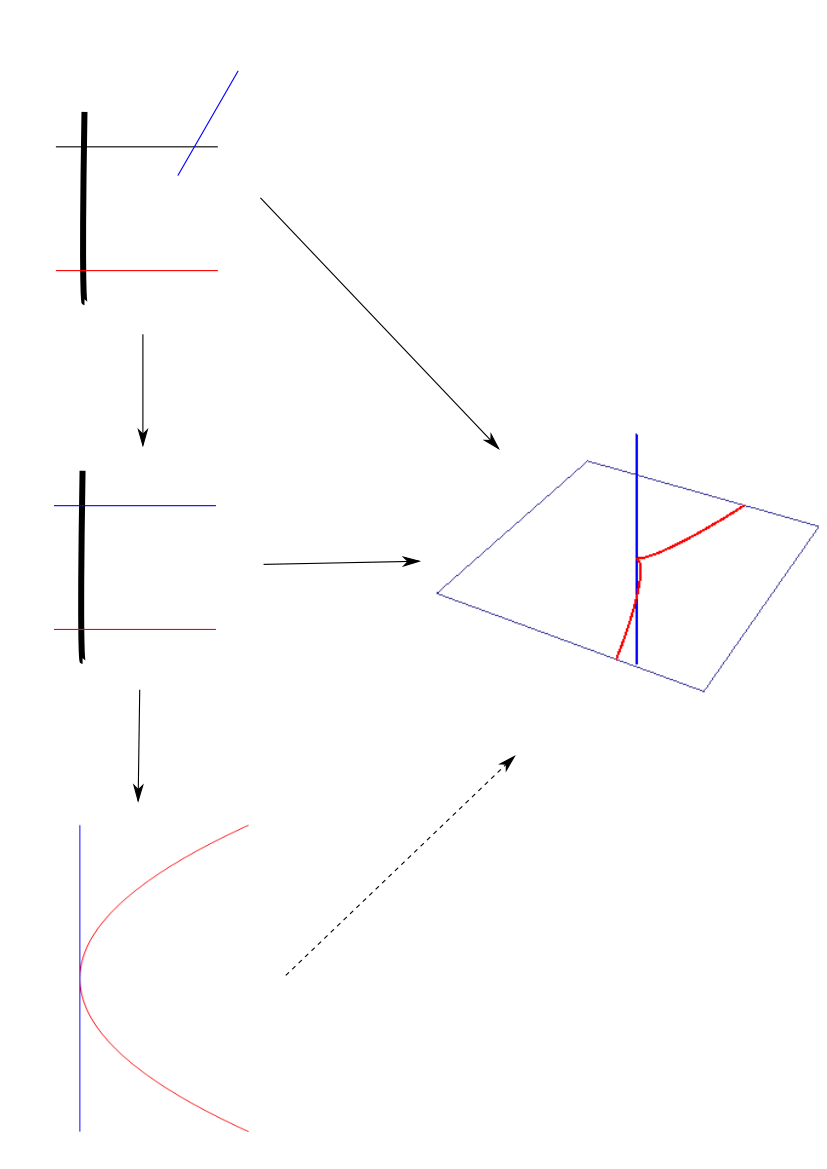
\includegraphics[width=10cm,height=5cm]{cusp_line_transv.png}
\end{center}

However, the argument can easily be fixed. Let $(\mathcal{C}_\eta,F_{\eta})$ be a stable map to $\PP^r$, defined on the generic point of a DVR scheme $S$; we may assume that $\mathcal C_{\eta}$ is smooth \cite[Section~3.2.1]{VISC}. 
As described in \cite[Step~1, Theorem~3.6]{VISC}, after applying nodal reduction we get a map $F\colon\mathcal C_S\to\PP^r_{S}$, for which we may suppose that $C_0$ is nodal and $f:=F_0$ is stable.

If $f$ is not constant on the minimal genus one sub-curve \cite{SMY1}, then it is also $m$-stable and there is nothing to say. Otherwise, let $E\subset C$ be the maximal connected genus one sub-curve where $f$ is constant and let $R_1\sqcup\dots\sqcup R_m=\overline{C/E}$.
 By Proposition~\ref{prop:components}(2) we know there is a non-trivial linear relation among the $\operatorname{d}\!f(T_{q_i}R_i)$'s.
 %In other words, the first derivatives of the sections $s_0,\dots,s_r$ defining $f$, satisfy a non trivial linear relation around $q_1,\dots,q_m =E\cup\bar{C/E}$.
 There are two possible situations:
 \begin{enumerate}
 \item $\operatorname{d}\!f(T_{q_i}R_i)\neq 0$ for every $i=1,\ldots,m$. Possibly after relabelling, this non-trivial relation looks like
 \[\alpha_1\operatorname{d}\!f(T_{q_{1}}R_{1})+\ldots +\alpha_j \operatorname{d}\!f(T_{q_{j}}R_{j})=0\]
  with all the coefficients being non-zero. Then, we may blow-up $\mathcal{C}$ in $q_{j+1},\ldots, q_m$. The induced map $\tilde{F_0}$ is constant on the exceptional divisors $E_{j+1},\ldots, E_m$, so we can complete the above linear relation to 
 \[\alpha_1\operatorname{d}\!\tilde f(T_{q_{1}}\tilde R_{1})+\ldots +\alpha_j \operatorname{d}\!\tilde f(T_{q_{j}}\tilde R_{j})+\beta_{j+1}\operatorname{d}\!\tilde f(T_{q_{j+1}}E_{j+1})+\ldots+\beta_m\operatorname{d}\!\tilde f(T_{q_{m}}E_m)=0\]
  with any choice of non-zero coefficients $\beta$. Now this \emph{sprouting} \cite[Section 2.3]{SMY2} ensures that the sections descend to the corresponding elliptic $m$-fold singularity. At this point, go to Step~2 of Viscardi's algorithm and follow it.
\item  
$\operatorname{d}\!f(T_{q_i}R_i)=0$ for some $i$, say for $i\in\left\{1,\dots,j\right\}$. 
 Then blow-up $\mathcal{C}$ at $q_{j+1},\ldots, q_m$. Observe that all $\operatorname{d}\!\tilde f(T_{q_i}R_i),\ i=1,\ldots,j$ and $\operatorname{d}\!\tilde f(T_{q_i}E_i),\ i=j+1,\ldots,m$ vanish, hence they satisfy any linear relation with non-zero coefficients, and they factorise through the corresponding singularity. The map has positive degree on the first $i=1,\ldots,j$ branches.
 \end{enumerate}
\end{remark}

The irreducible components of Viscardi's moduli space $\overline{\mathcal{M}}^m_{1,n}(\PP^r,\beta)$ are well understood too \cite[Thm.~5.9]{VISC}; indeed they have a similar description to the ones of Kontsevich' space. The main advantage of the $m$-stable compactification is that the number of components drops as $m$ increases.
 \begin{cor}\cite[Cor.~5.10]{VISC}
 For $m\geq\operatorname{min}(r,d)+n$, $\overline{\mathcal{M}}^m_{1,n}(\PP^r,\beta)$ is irreducible.
 \end{cor}


 Moreover, inspired by Viscardi's alternate compactification, we express a sufficient condition for smoothability in yet another way.
 \begin{prop}
Let $[f\colon C\to \PP^r]$ be a degenerate stable map from a ($n$-marked) genus one curve of the form $(E {}_{p_1,\ldots,p_m}\sqcup_{q_1,\ldots,q_m}\bigsqcup_{i=1}^m R_i,f)$, where $E$ is the maximal connected contracted arithmetic genus one subcurve, and $R_i$ are the rational tails (chains of $\PP^1$ along which $f$ has positive degree). 
 If $f$ factorises through a \emph{non-degenerate} (i.e. having positive degree along at least one of the branches of the singularity) map $f'\colon C'\to\PP^r$ from an elliptic $k$-fold singularity, with $k\leq m$, then  $\operatorname{d}\!f(T_{q_i}R_i)$ are linearly dependent in $T_{f(E)}\PP^r$.
 \end{prop}
 \begin{proof}
 Let $\xymatrix{C\ar[r]^{\pi} &C'\ar[r]^{f'} &\PP^r}$ be the factorization of $f$. Then $E'=\operatorname{Exc}(\pi)\subseteq E$ and 
  $\overline{C\setminus E'}=(S_1,q'_1)\sqcup\dots\sqcup (S_k,q'_k)\to (C',p)$ 
  is the normalization of the elliptic $k$-fold point. By hypothesis, $f=f'\circ\pi$ and $f$ is non-constant on $R_1,\dots R_m.$ Being $f'$ non-degenerate implies that there exists a subset
  $\left\{S_1,\ldots S_j\right\}\subseteq\left\{S_1,\ldots S_k\right\}$ 
  such that \[(S_1,q'_1)\cong (R_{i_1}, q_{i_1}),\ldots, (S_j,q'_j)\cong (R_{i_j}, q_{i_j}),\;\;\left\{i_1,\dots,i_j\right\}\subseteq \left\{1,\dots,m\right\}.\] 
By Smyth's characterisation of elliptic $k$-fold singularities, \cite[Lem.~2.2]{SMY1}, we obtain a non trivial linear relation 
  \begin{equation*}
  \label{eq:dep}\alpha_1\operatorname{d}\!\pi(T_{q_{i_1}}R_{i_1})+\ldots+\alpha_j \operatorname{d}\!\pi(T_{q_{i_j}}R_{i_j})+\alpha_{j+1}\operatorname{d}\!\pi(T_{q_{j+1}}S_{j+1})+\ldots+\alpha_k \operatorname{d}\!\pi(T_{q_k}S_k)=0
  \end{equation*}
  since all the coefficients are non-zero, $j\neq0$, and the second half of the formula can be ignored, we've got what we wanted.
  \end{proof}
\begin{rem}\label{remark:cuspunionline} 
The viceversa is not true, as Remark \ref{remark:sprouting} shows.
\end{rem}

In order to achieve the original goal of Gromov-Witten theory, i.e. the enumeration of smooth curves of genus $g$ in a target variety, mathematicians have been trying either to eliminate the unwanted components of Kontsevich's space (e.g. degenerate contributions from lower genus curves and multiple covers of lower degree curves) by defining alternate compactifications, or to concentrate the attention on the main component (i.e. find a suitable fundamental class supported on it). In genus one, Vakil and Zinger managed to do so by performing a sequence of blow-ups on an underlying space of weighted curves \cite{VZpreview} \cite{VZ} (see also \cite{HL}). The idea is that blowing up successively the locus of degree zero elliptic curve with one rational tail (\emph{elliptic tails}), then with two (\emph{elliptic bridges}), etc. and taking the fiber product
\bcd
\widetilde{\mathcal M}_{1,n}(\PP^r,d)\ar[r]\ar[d] & \M{1}{n}{\PP^r}{d}\ar[d] \\
\widetilde {\mathfrak M}_{1,n}^{\operatorname{wt}=d} \ar[r] & \mathfrak M_{1,n}^{\operatorname{wt}=d}
\ecd
the strict transform of the main component becomes smooth and meets the rest of the components in normal crossing fashion (the \'{e}tale local model being the union of two linear subspaces of different dimensions in affine space). Furthermore, the sheaves $\tilde\pi_*\tilde f^*\mathcal O_{\PP^r}(l)$ contain a vector subbundle of rank $dl$ supported on the strict transform of the main component. This paved the way to the definition of reduced invariants.
\begin{dfn}
Let $X$ be a complete intersection of degree $(l_1,\ldots,l_k)$ in $\PP^r$. The genus one \emph{reduced} Gromov-Witten invariants of $X$ are defined by integration on $$[\widetilde{\mathcal M}_{1,n}(\PP^r,d)^\circ]\cap c_{\operatorname{top}}(\tilde\pi_*\tilde f^*(\oplus_{i=1}^k\mathcal O_{\PP^r}(l_i))^\circ).$$
\end{dfn}

It is a matter of fact that the virtual dimension of the moduli space of maps to a three-fold $X$ is independent of the genus. In this context it was plausible to test the better enumerative properties of reduced invariants; in fact, Li-Zinger \cite{LZ} in the symplectic category and, later on, Chang-Li \cite{CL} in the algebraic one, proved a comparison formula for the quintic three-fold $X_5\subseteq\PP^4$ (or, more generally, for a complete intersection three-fold $X$ of degree $(l_1,\ldots,l_k)$ in $\PP^r$ with $\sum l_i\leq r+1$) of the form
$$GW_1(X)=\widetilde{GW}_1(X)+c\cdot GW_0(X).$$
We notice that the genus zero contribution to this formula comes from the boundary component with a single rational tail of degree $d$, while elliptic bridges and degenerate contributions with more rational tails do not matter to the genus one Gromov-Witten count. This suggests that removing the component with elliptic tails would provide a more direct and efficient definition of reduced invariants. We plan to do so by comparing the ordinary space of stable maps with Viscardi's space of 1-stable maps.

\section{Cuspidal curves and maps}

In this section we start investigating the Gromov- Witten type invariant obtained from Viscardi compactification studying the case $m=1$: the source curve is at worst cuspidal. We will see how in this case we can give a comparison with the GW-invariant and explain why the same technique does not work for higher $m$.
The first thing we do is the following:
we introduce a moduli space of stably-weighted, prestable, at worst cuspidal, marked curves. We show that there is a birational morphism from a correspondingly decorated moduli space of prestable nodal curves. Taking the fiber product with Viscardi's moduli space of stable cuspidal maps, we show that the resulting space includes in the usual Kontsevich's moduli space, precisely avoiding the component with elliptic tails $D_{\{d\},\{n\}}(X,d)$.

Why should such a morphism on decorated prestable curves exist? 
Consider an elliptic tail $C$; a one-dimensional family $\mathcal C$  with central fiber $\mathcal C_0\cong C$ will either be locally constant or smoothen the node. In the first case we can associate to this the locally constant family of cusps obtained by forgetting the elliptic tail and contracting a length-two infinitesimal neighborhood of the node in the rational component; in the second case, we claim that the line bundle $\mathcal O_\mathcal C(3q)$ gives a morphism to a smoothing of the cuspidal $\PP^1$. This heuristics (i.e. being able to substitute an elliptic tail with a cusp over points or DVR schemes) motivates us to believe we can define a morphism from suitably defined moduli spaces of nodal genus one curves to cuspidal curves (cfr. \cite[Lemma 4.2]{SMY2}). In fact we shall extend \cite[Corollary 4.5]{SMY2} to an appropriate setup of moduli stacks of weighted prestable curves. Assume $d>0$ throughout the following.

\begin{dfn}
Let $\mathfrak M_{1,n}^{\operatorname{wt}=d,\text{st}}$ be the stack of \emph{prestable} (projective, nodal and reduced), connected, arithmetic genus one, $n$-marked curves that are \emph{stably weighted} with total weight $d$, i.e. for every geometric point there is an integer-valued function on the set of irreducible components of the corresponding curve, such that it is compatible with specialisation maps and the sum of the integers is $d$; furthermore we require that all integers are nonnegative and every $p_a=0$ weight-0 component has at least three special points (every $p_a=1$ weight-0 component has at least one special point).
\end{dfn}
Remark that there is an \'{e}tale, non-separated morphism $\mathfrak M_{1,n}^{\operatorname{wt}}\to\mathfrak M_{1,n}$ and the weight stability condition is such that the forgetful map $\M{1}{n}{\PP^r}{d}\to\mathfrak M_{1,n}$ factorises through $\mathfrak M_{1,n}^{\operatorname{wt}=d,\text{st}}$, the weight assignment coming from the degree of the map to $\PP^r$.

\begin{dfn}
Let $\mathfrak M_{1,n}^{\operatorname{wt}=d,\text{st}}(1)$ be the stack of \emph{at worst cuspidal} projective, reduced, connected, arithmetic genus one, $n$-marked curves that are stably weighted with total weight $d$, i.e. as above with (stricter) stability condition: every $p_a=0$ weight-0 component has at least three special points (every $p_a=1$ weight-0 component has at least \emph{two} special point) \emph{and} every weight-0 cusp has at least two further special points.
\end{dfn}

Note that the only type of nodal curves that we are getting rid of is the one with an elliptic tail of weight zero.

\begin{thm}
There exists a morphism $\mathfrak M_{1,n}^{\operatorname{wt}=d,\text{st}}\to\mathfrak M_{1,n}^{\operatorname{wt}=d,\text{st}}(1)$ which extends the identity on the smooth locus.
\end{thm} 
We approach the proof in two different manners: first we adopt the strategy of constructing the graph of such morphism and prove that projection on the source is an isomorphism; second we construct the $1$-stabilisation at the level of curves with divisors with an argument \'{a} la Hassett \cite{HassettHyeon}, then argue that it descends to a morphism between moduli spaces of weighted curves.

\subsection{First approach: the graph}

Let $\mathcal C$ and $\mathcal C'$ be the universal curves over $\mathfrak{M}:=\mathfrak M_{1,n}^{\operatorname{wt}=d,\text{st}}$ and $\mathfrak{M}':=\mathfrak M_{1,n}^{\operatorname{wt}=d,\text{st}}(1)$ respectively. Abusing notation, we will still write $\mathcal C$ and $\mathcal C'$ for their pullbacks to the product $\mathfrak{M}\times\mathfrak{M}'$ along the two projections. The proof of the theorem follows from two Lemmas:

\begin{lem}\label{lemma:def_X}
 There is a locally closed substack $\mathcal X\subseteq\operatorname{Mor}_{\mathfrak{M}\times\mathfrak{M}'}(\mathcal C,\mathcal C')$ representing morphisms $C\to C'$ that contract weight-zero elliptic tails to cusps and are weight-preserving isomorphisms everywhere else. 
\end{lem}

\begin{lem}\label{lamma:projection_iso}
 The first projection $\pr_1\colon \operatorname{Mor}_{\mathfrak{M}\times\mathfrak{M}'}(\mathcal C,\mathcal C')\to\mathfrak M$ restricted to $\mathcal X$ is an isomorphism with $\mathfrak M$.
\end{lem}

\begin{proof}\ref{lemma:def_X}
Recall that $\operatorname{Mor}_{\mathfrak{M}\times\mathfrak{M}'}(\mathcal C,\mathcal C')$ is an algebraic stack; in fact the map to $\mathfrak{M}\times\mathfrak{M}'$ is representable (by algebraic spaces) \cite{OlssonHOM}. We now proceed to construct $\mathcal X$ as a locally closed substack in the space of morphisms.

\begin{description}[labelindent=0cm,leftmargin=\parindent]

\item[Step 1] Consider
 \[\pi\colon\mathfrak{P}=\mathfrak{Pic}^{tot deg=d,st}_{1,n}\to\mathfrak{M},\ \pi'\colon\mathfrak{P}'=\mathfrak{Pic}^{tot deg=d,st}_{1,n}(1)\to\mathfrak{M}'\]
  the Picard stacks of $\cC\to\mathfrak{M}$ and $\cC'\to\mathfrak{M'}$ with universal line bundles $\mathfrak{L}$ and $\mathfrak{L'}$, where $\pi$ and $\pi'$ are defined by taking the multi-degree of line bundles. We can now look at the algebraic stack $\operatorname{Mor}_{\mathfrak{P}\times\mathfrak{P}'}(\mathcal C,\mathcal C')$ with universal morphism
 $\Phi$ and natural projection $\Pi$ to $\operatorname{Mor}_{\mathfrak{M}\times\mathfrak{M}'}(\mathcal C,\mathcal C')$. We claim that there exists a locally closed substack $\mathcal{Y'}\subseteq \operatorname{Mor}_{\mathfrak{P}\times\mathfrak{P}'}(\mathcal C,\mathcal C')$ representing those morphisms that \emph{preserve the line bundles}. Indeed, given a chart 
 \begin{equation*}%\label{equation:Spoints} 
 S\to\operatorname{Mor}_{\mathfrak{P}\times\mathfrak{P}'}(\mathcal C,\mathcal C'),
  \end{equation*} 
   the locus of $s\in S$ where $\Phi_s^*\mathfrak{L}'_s\cong\mathfrak{L}_s$ is nothing else than the locus $T$ where the two sections $\mathfrak{L}_S$ and $\Phi_S^*\mathfrak{L}'_S$ of $\mathfrak{P}(S)\to\mathfrak{M}(S)$ coincide. In other words, we are looking at the fiber product 
  \[\xymatrix{T\ar[r]\ar[d]&\mathfrak{P}\ar[d]^{\Delta}\\
  S\ar[r]&\mathfrak{P}\times_{\mathfrak{M}}\mathfrak{P}}\]
Being $\mathfrak{P}\to\mathfrak{M}$ representable by locally separated algebraic spaces \cite[Theorem~8.3.1]{neron}, $\Delta$ is a quasi-compact locally closed immersion \cite[\href{http://stacks.math.columbia.edu/tag/04YU}{Tag 04YU}]{stacks-project}, so in particular $T\subseteq S$ is locally closed.

\item[Step 2] 
Furthermore there is a closed substack $\mathcal Y\subseteq \mathcal Y'$ representing \emph{surjective morphisms that preserve the markings}.

Given a chart $S\to\operatorname{Mor}_{\mathfrak{P}\times\mathfrak{P}'}(\mathcal C,\mathcal C')$, the locus of $s\in S$ where $\Phi_s$ is marking-preserving is the equaliser of the two sections
\bcd
S \ar[r,shift left, "\times\sigma_i'" above]\ar[r,shift right,"\times\Phi\circ\sigma_i" below] & \mathcal C_S'\times_S\ldots\times_S \mathcal C_S'
\ecd
This defines a closed subscheme of $S$, since $\mathcal C_S'\to S$ is separated.

As regards surjectivity, since $\Phi$ is proper and the dimension of the fiber is upper semicontinuous \cite[\href{http://stacks.math.columbia.edu/tag/0D4I}{Tag 0D4I}]{stacks-project}, the locus in $\mathcal C_S'$ where the fiber of $\Phi$ is empty is open. Its image in $S$ is open by flatness of $\cC'\to S$ \cite[\href{http://stacks.math.columbia.edu/tag/01UA}{Tag 01UA}]{stacks-project}, and the complement of it is the locus we need.
 
\item[Step 3] Let $\mathcal{X}'$ be the image of $\mathcal Y$ under $\Pi$. This is a constructible substack of $\operatorname{Mor}_{\mathfrak{M}\times\mathfrak{M}'}(\mathcal C,\mathcal C')$ by Chevalley's theorem \cite[Theorem 5.9.4]{LMB}. Recall that to show that a constructible set is open (respectively closed) it is enough to check that it contains all the generisations of its points (respectively all the specialisations) \cite[\href{http://stacks.math.columbia.edu/tag/0DQN}{Tag 0DQN}\href{http://stacks.math.columbia.edu/tag/0903}{Tag 0903}]{stacks-project}. Finally, under Noetherian assumptions, two points related by specialisation/generisation are contained in the image of a DVR scheme \cite[\href{http://stacks.math.columbia.edu/tag/054F}{Tag 054F}]{stacks-project}.

It is clear that being surjective and marking-preserving are closed conditions, as above. The requirement that $\phi$ can be covered by a line bundle-preserving map can be translated into the following combinatorial conditions:

\begin{enumerate}
\item\emph{$\phi$ contracts only weight zero components.} We show that this is open. Assume that $S$ is a DVR scheme with closed point $0$ and generic point $\eta$, and we are given $S\to\mathcal X'$ such that $\phi_0\colon\mathcal C_0\to \mathcal C_0'$ does not contract any positive weight component. Suppose there exists an irreducible component $D_\eta\subseteq C_{\eta}$ of positive weight $d_W$ which is contracted by $\phi_{\eta}.$ The contracted locus, i.e. $\left\{c\in \mathcal{C}_{S} | \dim_c\phi^{-1}(\phi(c))\geq 1\right\}$, is closed by semicontinuity of fiber dimension, hence it contains all the components $D_i\subseteq C_0$ to which $D_\eta$ specialises. At least one of them has positive weight, since the sum of their weights is $d_W$, which is a contradiction.

\item\emph{$\phi$ has degree 1 on every non contracted component} or, equivalently, there is an $S$-dense open in $\mathcal C'_S$ such that the restriction of $\phi_S$ to its preimage is an isomorphism.
This is an open and closed condition; we show it is open. Let $S$ be a DVR scheme as above and assume that $\phi_0$ satisfies the property. Since $\phi_S$ is proper, we may consider 
\[\phi_{S,*}[\mathcal C_{S}]=\sum n_i[\mathcal C'_{S,i}]\in A_2(\cC'_S)\]. Applying Gysin pull-back to $0$ (which is a regular closed point of the base) \cite[Prop. 10.1(a)]{FUL}, we see that all the $n_i$'s are 1 for those $\cC'_i$'s such that $0^![\cC'_i]\neq 0$. On the other hand there is no irreducible component of $\cC'$ supported on $\cC'_\eta$.

\item\emph{$\phi$ is weight-preserving.} This is again an open condition, as we can see from the weighted dual graphs. Let $\tilde \phi$ be the map induced at the level of weighted dual graphs $\Gamma(\cC)\to\Gamma(\cC')$. It is compatible with the specialisation maps:
\bcd
\Gamma(\cC_0)\ar[r,"\tilde\phi_0"]\ar[d,"\rm{sp}"] & \Gamma(\cC'_0)\ar[d,"\rm{sp}"] \\
\Gamma(\cC_{\eta})\ar[r,"\tilde\phi_\eta"]& \Gamma(\cC'_\eta)
\ecd
Since the weight of a component of the generic fiber is determined by those of the components to which it specialises
\[ \deg(v)=\sum_{w\in\rm{sp}^{-1}(v)}\deg(w)
\]
$\tilde{\phi}_\eta$ has to be weight-preserving as well.
\end{enumerate}

\item[Step 4] We have seen that, if $\phi$ contracts a connected subcurve $E$ of the fiber, it must have zero weight. Since the target only has nodes and cusps as singularities, and the markings are required to be smooth points, we observe that $E$ must be of arithmetic genus one by weighted stability and $|\overline{C\setminus E}\cap E|\leq 2$, i.e. $E$ is either an elliptic tail or an elliptic bridge. There are basically two possibilities:
\begin{enumerate}
\item $\phi$ contracts an elliptic tail to a cusp and is an isomorphism everywhere else, or there is no elliptic tail to start with and $\phi$ is an isomorphism;
\item the elliptic tail/bridge is contracted to a smooth point/node, then a non-separating node or a cusp must be created somewhere else in order to preserve the arithmetic genus.
\end{enumerate} 
We want to avoid the second scenario, so we define the open substack $\mathcal X\subseteq \mathcal X'$ as follows.
Given $\mathcal{C}_S\to\mathcal C_S'\in\mathcal X'(S)$, let $U'\subseteq \mathcal C'$ be the \emph{maximal} $S$-dense open subset such that $\phi_S|_{\phi_S^{-1}(U')}\colon\phi_S^{-1}(U')\to U'$ is an isomorphism and $Z'$ its closed complement in $\mathcal C_S'$. 
Then $\mathcal X$ is the open locus \cite[\href{http://stacks.math.columbia.edu/tag/055G}{Tag 055G}]{stacks-project} where the fibers of $\pi|_{\phi^{-1}(Z')}\colon \phi^{-1}(Z')\to S$ are geometrically connected.
\end{description} 
 \end{proof}
 
 \begin{proof}\ref{lamma:projection_iso}
 This result will follow from an application of Zariski's Main Theorem for algebraic spaces.
First we claim that the projection is \emph{representable by algebraic spaces}: by \cite[\href{http://stacks.math.columbia.edu/tag/04Y5}{Tag 04Y5}]{stacks-project} we only need to check that it is faithful, and by \cite[Theorem 2.2.5]{CONR} it is enough to look at geometric points. Hence we need to say that, given $\phi\colon C\to C'$ a $k$-point of $\X$, we have
$\operatorname{Aut}(\phi)\subseteq\operatorname{Aut}(C)$. Recall that automorphisms of $\phi$ are commutative diagrams:
\bcd C\ar[r,"\phi"]\ar[d,"\psi"] & C'\ar[d,"\psi'"] \\ C\ar[r,"\phi"] & C' \ecd
 Now $\psi'$ is determined by $\psi$ due to our description of $\phi$.
 
Secondly $\pr_{1|\mathcal X}$ is \emph{proper}: this can be seen using the valuative criterion
\bcd
\eta'=\Spec(K')\ar[r]\ar[d] & \eta=\Spec(K)\ar[r]\ar[d] & \mathcal X \ar[d] \\
S'=\Spec(R')\ar[r]\ar[urr,dashed,"\exists?", left] & S=\Spec(R)\ar[r] & \mathfrak M
\ecd
Let $\pi \colon \mathcal C_S\to S$ be the family of nodal curves on $S$; there are three cases to consider:
\begin{enumerate}
\item the central fiber contains no elliptic tail, then the same is true for $\mathcal C_\eta$, hence $\phi_\eta$ is an isomorphism. We can extend $\phi_\eta$ as follows:
\bcd
\cC_\eta\arrow{r}{\sim}[swap]{\phi_\eta}\ar[d,hook,"\iota"] & \cC'_\eta\ar[d,hook,"\iota\circ\phi_\eta^{-1}"] \\
\cC_S\ar[r,"\id_\cC"] & \cC_S=:\cC'_S
\ecd
Another extension $\phi'\colon \mathcal C_S\cong \mathcal C_S'$ would be isomorphic to the previous one via:
\bcd
\cC_S\ar[r,"\phi'"]\ar[d,"\id"] &\cC_S'\ar[d,"(\phi')^{-1}"] \\
\cC_S\ar[r,"\id"] & \cC_S
\ecd

\end{enumerate}
If instead $\mathcal C_0$ has got an elliptic tail, then we have two possibilities:
\begin{enumerate}
\setcounter{enumi}{1}
\item $\mathcal C_{\eta}$ has an elliptic tail as well; that is the image of $S\to\MM$ is contained in the boundary, so we can find a lift
\bcd
 & \MM_{1,1}\times\MM_{0,1+n}^\text{wt}\ar[d] & \\
 S\ar[r]\ar[ur,dashed] & \mathfrak D_{\{1,\emptyset\},\{0,n\}}\ar[r,hook] &\MM.
\ecd
 Then $\mathcal C_S$ is the push-out of a family of rational curves $\mathcal R_S$ and a family of genus one curves $\mathcal Z_S$:
%The map $S\to\partial \mathfrak M_{1,n}$ lifts to the normalisation of the boundary, i.e. $\mathfrak M_{0,n_0+1}\times\mathfrak M_{1,n_1+1}$, which gives two families of pointed curves on $S$; there is a map from the push-out to $\mathcal C_S$ by the universal property, and it is proper bijective and flat (crit\`{e}re de platitude par fibres \cite[\href{http://stacks.math.columbia.edu/tag/039A}{Tag 039A}]{stacks-project}).
\begin{equation}\label{eq:pushout}
\begin{tikzcd}
S\ar[d]\ar[r] & \mathcal R_S \ar[d] \\
\mathcal Z_S\ar[r] & \mathcal C_S
\end{tikzcd}
\end{equation}
Recall that the cuspidal curve $\cC'_K$ can be characterised as the push-out of the following diagram:
\bcd
2K\ar[r]\ar[d] & \mathcal R_K\ar[d] \\
K\ar[r] & \mathcal C'_K.
\ecd
Since the smooth section $S\to\mathcal R_S$ defines a Cartier divisor, it makes sense to take its double and we can thus define $\cC'_S$ by means of the similar diagram:
\bcd
2S\ar[r]\ar[d] & \mathcal R_S\ar[d] \\
S\ar[r] & \mathcal C'_S
\ecd
The morphism $\phi_S\colon\cC_S\to\cC'_S$ extending $\phi_\eta$ is then defined by exploiting the description of $\cC_S$ as a push-out \eqref{eq:pushout}, and the morphisms $\id\colon\mathcal R_S\to \mathcal R_S$ and $\pr_{\mathcal Z_S}\colon\mathcal Z_S\to S$.
\item If $\mathcal C_S$ smoothens the elliptic tail, then $\phi_\eta$ is an isomorphism. We may assume that $S$ is the spectrum of a complete DVR with algebraically closed residue field \cite[Theorem 7.10]{LMB}. Then we may pick one smooth section for each rational component of $\cC_0$ and extend them to sections of $\cC_S\to S$ by Grothendieck's existence theorem; let us denote by $\Sigma$ the Cartier divisor that is the sum of all such sections. Let $Z$ be the elliptic tail in the central fiber; then we claim that $\omega_{\cC_S/S}(Z)\otimes\mathcal O_{\cC_S}(\Sigma)$ is $\pi_S$ semi-ample, ample on the generic fiber, and gives the contraction of the elliptic tail to the cusp in the central fiber. We shall not prove the claim here, since this is the core of the second approach.
\end{enumerate}
Finally, observe that the map is bijective by construction and $\mathfrak M$ is normal, hence $\pi_{|\mathcal X}\colon\mathcal X\to \mathfrak M$ is an isomorphism by Zariski's main theorem (as in \cite[\href{http://stacks.math.columbia.edu/tag/082I}{Tag 082I}]{stacks-project}).
 \end{proof}
\subsection*{Why only cusps?} 
\subsection*{Alternative constructions}
\begin{itemize}
\item adapt the ideas of \cite{HassettHyeon}: check out section 3 of this paper;
\item check \cite[\S 4]{RSPW}.
\end{itemize}
 \section{Comparison with $p$-fields and splitting}
\subsection{Notation}
Let $\Z$ be defined by the pullback diagram:
\bcd
\mathcal Z \ar[r]\ar[d]\ar[rd,phantom,"\Box"] & \overline{\mathcal M}_1^{(1)}(\PP^4,d) \ar[d] \\
\mathcal X\ar[r] & \mathfrak M_1^{(1)}
\ecd

Objects of $\Z$ over $S$ consist of diagrams
\bcd
\cC\ar[rr,"\phi"]\ar[dr,"\pi"] & & \hat\cC\ar[rr,"f"]\ar[dl,"\hat\pi"] & & \PP^4 \\
& S & & &
\ecd
where $f$ is a $1$-stable map and $\phi$ is the weighted $1$-stabilisation (i.e. contraction of elliptic tails of weight $0$); arrows over $\id_S$ are commutative diagrams
\bcd
\cC\ar[r,"\phi"]\ar[d,"\psi"] &  \hat\cC\ar[r,"f"]\ar[d,"\hat\psi"] & \PP^4 \ar[d,"\id_\PP"]\\
\cC'\ar[r,"\phi'"] &  \hat\cC'\ar[r,"f'"] & \PP^4

\ecd
where $\psi$ and $\hat\psi$ are isomorphisms; note once again that $\hat \psi$ is determined by $\psi$, due to the required commutativity with the dominant ``birational'' morphism $\phi$.

Forgetting $\hat \cC$ and keeping $f\circ\phi\colon \cC\to\PP^4$, we obtain a morphism $i\colon\Z\to\oM_1(\PP^4,d)$, which we claim is a \emph{closed embedding}: in fact, from the above description of arrows in $\Z$, it is representable (i.e. faithful) and a proper (check the valuative criterion: use the fact that $\X\to\MM_1$ is proper, and the map to $\PP$ descends to the $1$-stabilisation because we are only contracting weight $0$ elliptic tails; compare with \cite[Theorem 4.3]{RSPW}) monomorphism (i.e. full). So we may add the commutative diagram to the left:
\bcd
\oM_1(\PP^4,d)\ar[d] & \mathcal Z \ar[l,swap,hook,"i"]\ar[r]\ar[d]\ar[rd,phantom,"\Box"] & \overline{\mathcal M}_1^{(1)}(\PP^4,d) \ar[d] \\
\MM_1 & \mathcal X\ar[l,swap,"\sim"]\ar[r] & \mathfrak M_1^{(1)}
\ecd

\begin{lem}
There is a closed embedding $i\colon\Z\hookrightarrow\oM_1(\PP^4,d)$. In particular $\Z$ is a proper DM stack.
\end{lem}

Furthermore we inherit a description of the irreducible components of $\Z$: there is a main component $\Z^\text{main}$ which is the closure of the locus of maps from a smooth elliptic curve, and for every $k\geq 2$ a boundary component $D^k\Z$, whose general point represents a contracted elliptic curve with $k$-many rational tails of positive degree. Notice that the above lemma signifies that each and every component of $\Z$ is isomorphic to the corresponding one in $\oM_1(\PP^4,d)$. The point is that given any stable map there is at most one factorisation through the weighted $1$-stabilisation of the curve: objects of $\oM_1(\PP^4,d)\setminus D^1$ are $1$-stable already; objects of $D^1\cap \oM_1(\PP^4,d)^\text{main}$ do factor thanks to Vakil's criterion and objects of $D^1\cap D^k$ ($k\geq 2$) do factor through a map which is constant on the cusp.\marginpar{insert figure of a typical element of $D^1\cap D^2$.} On the other hand, objects of $D^{1,\circ}=D^1\setminus(\oM_1(\PP^4,d)^\text{main}\cup\bigcup_{k\geq 2}D^k)$ do not admit any factorisation, so that $\Z$ has no corresponding component.

\textcolor{red}{Introduce a Hu-Li type blow-up of $\MM_1^{(1)}$.}

We can push this reasoning further to the level of $p$-fields:
\bcd
\oM_1(\PP^4,d)^p\ar[d] & \mathcal Z^p \ar[l,swap,hook,"j"]\ar[r]\ar[d]\ar[rd,phantom,"\Box"] & \overline{\mathcal M}_1^{(1)}(\PP^4,d)^p \ar[d] \\
\oM_1(\PP^4,d)\ar[d] & \mathcal Z \ar[l,swap,hook,"i"]\ar[r]\ar[d]\ar[rd,phantom,"\Box"] & \overline{\mathcal M}_1^{(1)}(\PP^4,d) \ar[d] \\
\MM_1 & \mathcal X\ar[l,swap,"\sim"]\ar[r] & \mathfrak M_1^{(1)}
\ecd
where this time an object of $\Z^p$ over $S$ is given by
\bcd
\cC\ar[rr,"\phi"]\ar[dr,"\pi"] & & \hat\cC\ar[rr,"f"]\ar[dl,"\hat\pi"] & & \PP^4 & \text{and} & \xi\in\Gamma(\hat\cC,f^*\OO_\PP(-5)\otimes\omega_{\hat\cC/S}) \\
& S & & & & &
\ecd
(I think to satisfy the stack condition $\xi$ should be really thought of as a section of $\hat\pi_*(f^*\OO_\PP(-5)\otimes\omega_{\hat\cC/S})$.)

For the existence of $j$ we are claiming that, pulling back along $\phi$, $\xi$ induces a section of $\pi_*((f\circ\phi)^*\OO_\PP(-5)\otimes\omega_{\cC/S})$. We may work on an atlas for $\Z^p$, which we shall (maybe abusing notation slightly) denote by $S$, as the base scheme in the above diagram; let us also denote by $\hat{\mathcal L}=f^*\OO(1)$ and $\L=\phi^*\hL$.

First we claim that the adjunction map $\OO_{\hat\cC}\to\phi_*\OO_\cC$ is an isomorphism: it is injective by dominance of $\phi$; to check the cokernel is trivial it is enough to do so after restricting to each and every irreducible component of $\Z^p$. Then $\hat\cC$ is normal\marginpar{NO, $\hat\cC_{|D^k}$ has multiple components} (so is the base\footnote{on VZ here}; R1 follows from the fact that singularities are isolated in the fiber, S2 \footnote{OK when fibers are Cartier i.e. over a DVR; actually take a look at Thm 23.9 in Matsumura's Commutative Ring Theory, fibers are CM in the situation at hand } follows from reducedness of the fibers) and we conclude by Zariski's main theorem (geometric fibers of $\phi$ are either points or elliptic curves, in either case connected).

The equality $\phi^*\omega_{\hat\cC/S}=\omega_{\cC/S}(\mathcal E)$, where $\mathcal E$ is the locus spanned by elliptic tails, can be checked on $\X$ and then pulled back. Notice that $\mathcal E$ is a Cartier divisor; $\phi$ is generically an isomorphism, so $\phi^*\omega_{\hat\cC/S}$ and $\omega_{\cC/S}$ may differ only on the locus where $\phi$ is not an isomorphism. The statement may now be proved by an intersection-theoretic argument by reducing to smoothings over the spectrum of a DVR, see\cite[Lemma 2.13]{SMY1}.

It is clear now that $\omega_{\cC/S}\otimes\L^{\otimes -5}\hookrightarrow \phi^*(\omega_{\hat\cC/S}\otimes\hL^{\otimes-5})$. Pushing down along $\pi=\hat\pi\circ\phi$, we get a map $\pi_*(\omega_{\cC/S}\otimes\L^{\otimes -5})\hookrightarrow \hat\pi_*(\omega_{\hat\cC/S}\otimes\hL^{\otimes-5})$ (using the projection formula and $\phi_*\OO_\cC=\OO_{\hat\cC}$). These are both $0$ on $\Z^{\text{main},\circ}=\Z^\text{main}\setminus(\bigcup_{k\geq2} D^k\Z)$; on the other hand they are both line bundles on $D^k\Z$... \marginpar{Fix me}

\begin{lem}
There is a close embedding $j\colon \Z^p\hookrightarrow \oM_1(\PP^4,d)^p$.
\end{lem}

Notice that the $p$-field is forced to vanish on $\Z^{\text{main},\circ}$, so $(\Z^p)^{\text{main},\circ}\simeq\Z^{\text{main},\circ}$ is the zero-section of the cone $\Z^p\to\Z$ (even though $\oM_1(\PP^4,d)^p\to \oM_1(\PP^4,d)$ is non-trivial on $\oM_1(\PP^4,d)^\text{main}\cap D^1$).

Finally it will be useful to introduce
\bcd
\XP\ar[r]\ar[d]\ar[dr,phantom,"\Box"] & \mathfrak{Pic}_1^{(1)}\ar[d] \\
\X\ar[r] & \MM_1^{(1)}
\ecd
so that objects of $\XP(S)$ are
\bcd
\cC\ar[rr,"\phi"]\ar[dr,"\pi"] & & \hat\cC\ar[dl,"\hat\pi"] & \text{and} & \hL\in\Pic_{\hat \cC/S}(S) \\
& S & & &
\ecd
Notice that the map $\XP\to\mathfrak{Pic}$ that associates to an object as above $(\cC\to S,\phi^*\hL)$ is highly non-trivial on the locus of elliptic tails/cusps, since
\begin{itemize}
\item line bundles of the same degree on the cusp are identified (there is a $\mathbb G_a$ wealth of them), and
\item only line bundles that restrict to effective line bundles on the elliptic tail are in the image of this morphism.
\end{itemize}

\subsection{Splitting the cone}
We may notice that $(\Z^p)^{\text{main},\circ}\to\XP$ is smooth onto its image, which is an open substack; furthermore on this open the relative tangent is represented by $\hat\pi_*\hL^{\oplus 5}$, and $\R^1\hat\pi_*\hL^{\oplus 5}=\hat\pi_*(\hat\omega\otimes\hL^{\otimes -5})=0$. Let $E^\bullet=\R^\bullet\hat\pi_*(\hL^{\oplus 5}\oplus \hat\omega\otimes\hL^{\otimes -5})$ denote the dual perfect obstruction theory of $\Z^p\to \XP$. Then the intrinsic normal cone of $\Z^p\to \XP$ splits into:
\begin{itemize}
\item the closure of the zero section of $h^1/h^0(E^\bullet)_{|\text{main},\circ}$, which we shall name $\mathfrak C^{\text{main}}$;
\item other components supported on the boundary, which we should accordingly name $\mathfrak C^k$ ($k\geq 2$).
\end{itemize}
\bibliographystyle{alpha}
\bibliography{cusp}

\end{document}
